\section{Results}

\subsection{Primary Outcome: Production Validation Acceptance}
Across all 604 prompt-level trials (151 prompts for each of four models), single-shot production validation succeeded for 309/604 cases (51.16\%). Under validator-in-the-loop refinement, pipeline production validation succeeded for 604/604 cases (100.00\%).

\begin{figure}[H]
\centering
% Figure 2 options (pick one):
% \definecolor{singleShotColor}{RGB}{196,106,28}
\definecolor{pipelineColor}{RGB}{44,138,100}
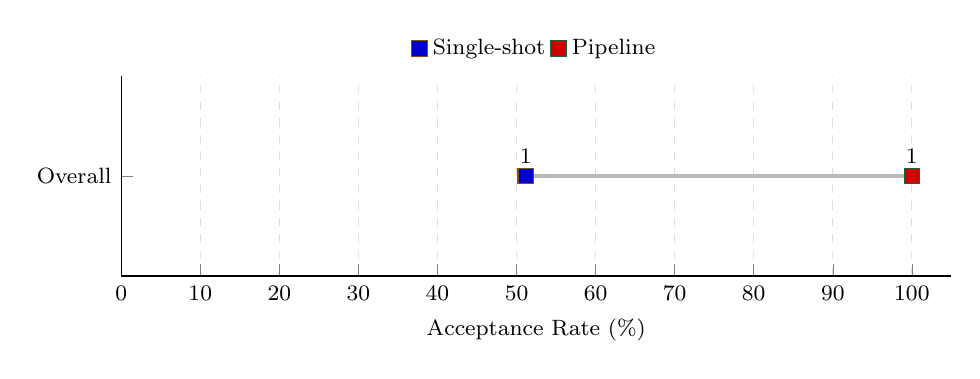
\begin{tikzpicture}
\begin{axis}[
    width=\columnwidth,
    height=0.34\columnwidth,
    xmin=0,
    xmax=105,
    ymin=0.4,
    ymax=1.6,
    xlabel={Acceptance Rate (\%)},
    ytick={1},
    yticklabels={Overall},
    axis lines*=left,
    xmajorgrids=true,
    grid style={dashed,gray!25},
    tick label style={font=\footnotesize},
    label style={font=\footnotesize},
    legend style={
        draw=none,
        font=\footnotesize,
        at={(0.5,1.03)},
        anchor=south,
        legend columns=2
    }
]
\addplot+[very thick,gray!55,mark=none,forget plot] coordinates {(51.16,1) (100.00,1)};

\addplot+[
    only marks,
    mark=square*,
    mark size=2.8pt,
    fill=singleShotColor,
    draw=singleShotColor!70!black,
    nodes near coords,
    nodes near coords style={font=\footnotesize, text=black, anchor=south, yshift=1pt},
] coordinates {(51.16,1)};

\addplot+[
    only marks,
    mark=square*,
    mark size=2.8pt,
    fill=pipelineColor,
    draw=pipelineColor!70!black,
    nodes near coords,
    nodes near coords style={font=\footnotesize, text=black, anchor=south, yshift=1pt},
] coordinates {(100.00,1)};

\legend{Single-shot,Pipeline}
\end{axis}
\end{tikzpicture}

% \definecolor{singleShotColor}{RGB}{196,106,28}
\definecolor{pipelineColor}{RGB}{44,138,100}
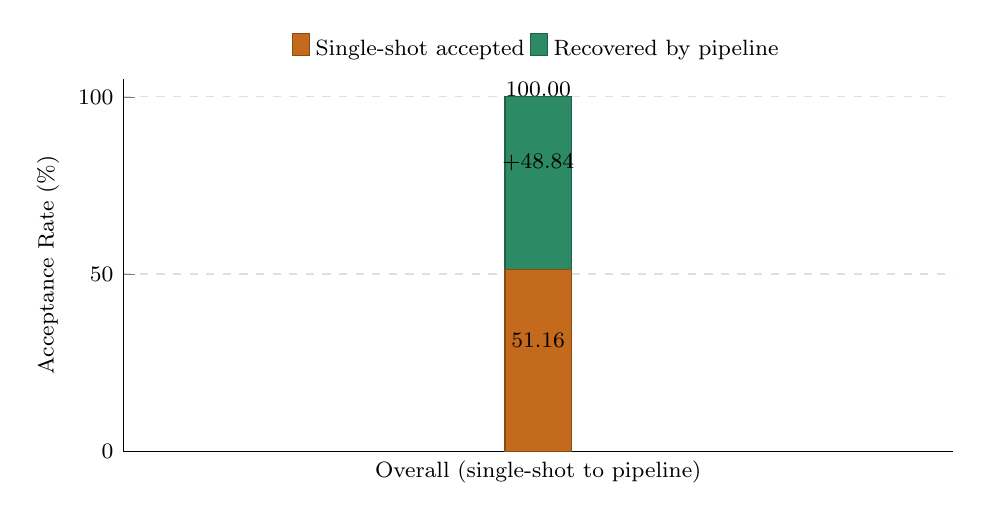
\begin{tikzpicture}
\begin{axis}[
    ybar stacked,
    bar width=24pt,
    width=\columnwidth,
    height=0.52\columnwidth,
    ymin=0,
    ymax=105,
    ylabel={Acceptance Rate (\%)},
    symbolic x coords={Overall},
    xtick=data,
    xticklabels={Overall (single-shot to pipeline)},
    x tick label style={font=\footnotesize, align=center},
    axis lines*=left,
    ymajorgrids=true,
    grid style={dashed,gray!25},
    tick label style={font=\footnotesize},
    label style={font=\footnotesize},
    legend style={
        draw=none,
        font=\footnotesize,
        at={(0.5,1.02)},
        anchor=south,
        legend columns=2
    },
]
\addplot+[
    fill=singleShotColor,
    draw=singleShotColor!70!black,
    nodes near coords,
    every node near coord/.append style={font=\footnotesize, text=black, anchor=south, yshift=1pt},
] coordinates {(Overall,51.16)};

\addplot+[
    fill=pipelineColor,
    draw=pipelineColor!70!black,
    nodes near coords,
    every node near coord/.append style={font=\footnotesize, text=black, anchor=south, yshift=1pt},
    point meta=explicit symbolic,
    nodes near coords={+\pgfmathprintnumber[fixed,precision=2]{\pgfplotspointmeta}},
] coordinates {(Overall,48.84) [48.84]};

% Top label (pipeline total)
\node[font=\footnotesize] at (axis cs:Overall,102.0) {100.00};

\legend{Single-shot accepted,Recovered by pipeline}
\end{axis}
\end{tikzpicture}

\definecolor{singleShotColor}{RGB}{196,106,28}
\definecolor{pipelineColor}{RGB}{44,138,100}
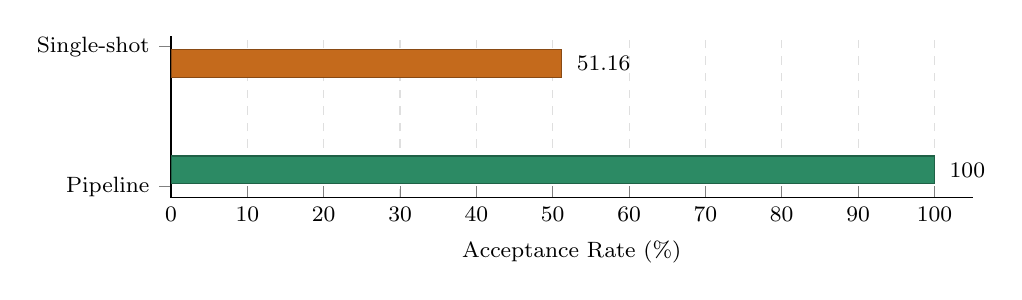
\begin{tikzpicture}
\begin{axis}[
    xbar,
    width=0.97\columnwidth,
    height=0.30\columnwidth,
    xmin=0,
    xmax=105,
    xlabel={Acceptance Rate (\%)},
    symbolic y coords={Pipeline,Single-shot},
    ytick={Single-shot,Pipeline},
    yticklabels={Single-shot,Pipeline},
    enlarge y limits={abs=4pt},
    axis lines*=left,
    xmajorgrids=true,
    grid style={dashed,gray!25},
    tick label style={font=\footnotesize},
    label style={font=\footnotesize},
    nodes near coords,
    every node near coord/.append style={font=\footnotesize, text=black, anchor=west, xshift=2pt},
]
\addplot+[fill=singleShotColor, draw=singleShotColor!70!black] coordinates {
    (51.16,Single-shot)
};
\addplot+[fill=pipelineColor, draw=pipelineColor!70!black] coordinates {
    (100.00,Pipeline)
};
\end{axis}
\end{tikzpicture}

\caption{Overall single-shot vs final pipeline production-validation acceptance across all 604 prompt-level cases.}
\label{fig:overall_baseline_vs_pipeline}
\end{figure}

\subsection{Per-Model Reliability}
All models reached 151/151 eventual production validation under the validator-gated loop, but single-shot pass rates differed substantially. Figure~\ref{fig:by_model_baseline_vs_pipeline} provides the per-model comparison with exact acceptance values annotated on the bars.

\begin{figure}[H]
\centering
\definecolor{singleShotColor}{RGB}{196,106,28}
\definecolor{pipelineColor}{RGB}{44,138,100}
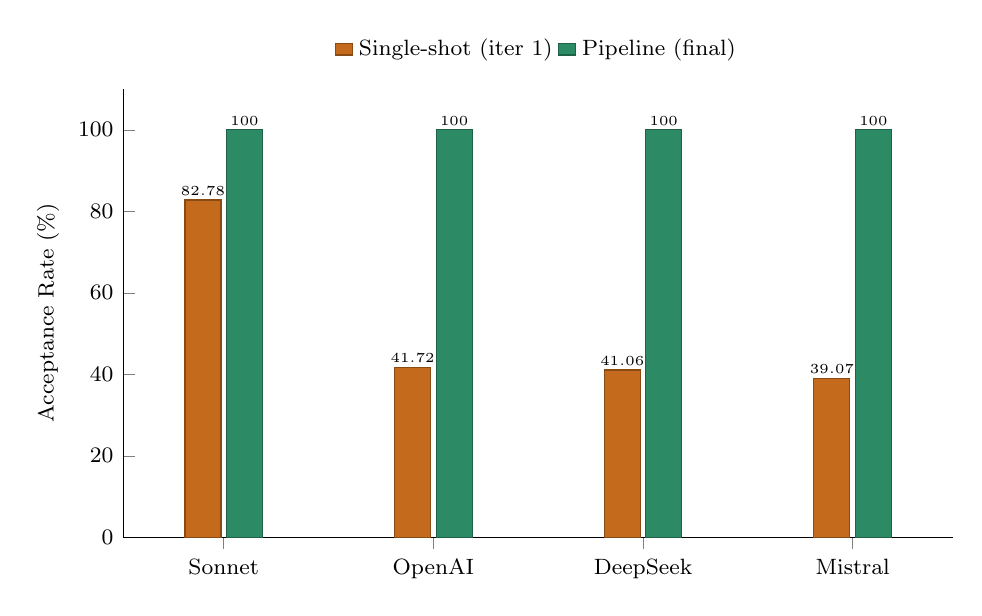
\begin{tikzpicture}
\begin{axis}[
    ybar,
    bar width=13pt,
    width=\columnwidth,
    height=0.60\columnwidth,
    ymin=0,
    ymax=110,
    ylabel={Acceptance Rate (\%)},
    symbolic x coords={Sonnet,OpenAI,DeepSeek,Mistral},
    xtick=data,
    xticklabel style={font=\footnotesize, rotate=0, anchor=north},
    nodes near coords,
    nodes near coords={\pgfmathprintnumber[fixed,precision=2]{\pgfplotspointmeta}},
    nodes near coords align={center},
    nodes near coords style={
        font=\tiny,
        text=black,
    },
    every node near coord/.append style={anchor=south, yshift=-1.8pt},
    ymajorgrids=false,
    enlarge x limits=0.16,
    axis lines*=left,
    tick label style={font=\footnotesize},
    label style={font=\footnotesize},
    legend style={
        draw=none,
        font=\footnotesize,
        at={(0.5,1.04)},
        anchor=south,
        legend columns=2
    },
    legend cell align={left},
    legend image code/.code={
        \draw[#1] (0cm,-0.075cm) rectangle (0.22cm,0.075cm);
    },
]
\addplot+[fill=singleShotColor, draw=singleShotColor!70!black] coordinates {
    (Sonnet,82.78)
    (OpenAI,41.72)
    (DeepSeek,41.06)
    (Mistral,39.07)
};
\addplot+[fill=pipelineColor, draw=pipelineColor!70!black] coordinates {
    (Sonnet,100.00)
    (OpenAI,100.00)
    (DeepSeek,100.00)
    (Mistral,100.00)
};
\legend{Single-shot (iter 1),Pipeline (final)}
\end{axis}
\end{tikzpicture}

\caption{Per-model single-shot vs final pipeline production-validation acceptance.}
\label{fig:by_model_baseline_vs_pipeline}
\end{figure}

Anthropic Sonnet 4.6 had the highest single-shot pass rate (82.78\%), while OpenAI (41.72\%), DeepSeek Reasoner (41.06\%), and Mistral Large (39.07\%) showed worse single-shot behavior and larger single-shot-to-pipeline gaps.

\subsection{Convergence Behavior}
Convergence is indexed by repair cycles: $k=0$ denotes the initial single-shot generation (no validator feedback), and $k\geq 1$ denotes validator-guided repair cycles; acceptance corresponds to zero-error output under the production validator.

Figure~\ref{fig:cumulative_convergence} first presents the pooled convergence trajectory across all prompt-level cases.

\begin{figure}[H]
\centering
\definecolor{pipelineColor}{RGB}{44,138,100}
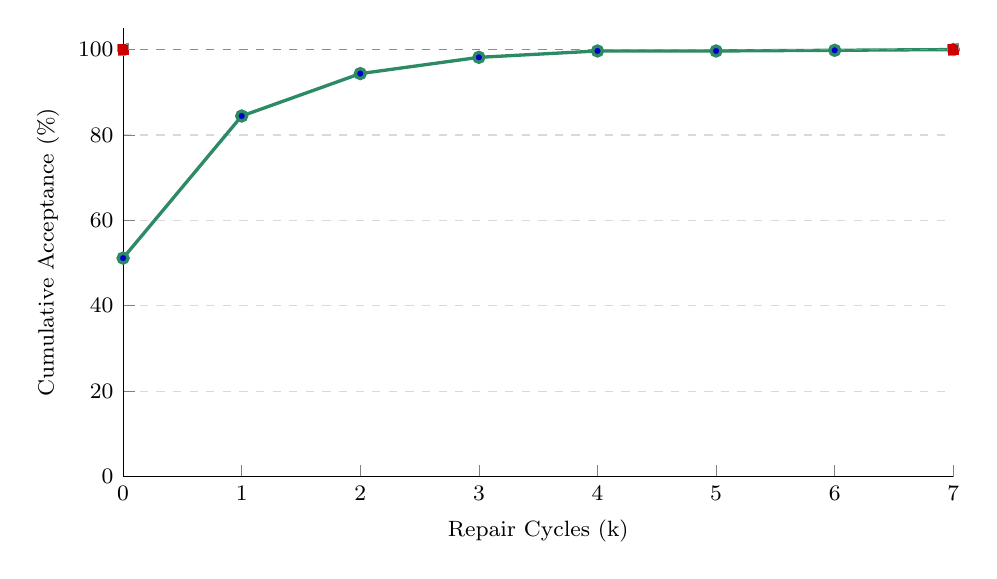
\begin{tikzpicture}
\begin{axis}[
    width=\columnwidth,
    height=0.60\columnwidth,
    xmin=0,
    xmax=7,
    ymin=0,
    ymax=105,
    xlabel={Repair Cycles (k)},
    ylabel={Cumulative Acceptance (\%)},
    xtick={0,1,2,3,4,5,6,7},
    ymajorgrids=true,
    xmajorgrids=false,
    grid style={dashed,gray!30},
    axis lines*=left,
    tick label style={font=\footnotesize},
    label style={font=\footnotesize},
]
\addplot+[pipelineColor, very thick, mark=*, mark size=1.8pt] coordinates {
    (0,51.16)
    (1,84.44)
    (2,94.37)
    (3,98.18)
    (4,99.67)
    (5,99.67)
    (6,99.83)
    (7,100.00)
};
\addplot+[black!45, dashed, thin] coordinates {(0,100) (7,100)};
\end{axis}
\end{tikzpicture}

\caption{Cumulative production-validation acceptance versus repair cycles ($k$). $k=0$ denotes initial single-shot generation; $k\geq 1$ denotes validator-guided repair cycles. Acceptance corresponds to zero-error output under the production validator.}
\label{fig:cumulative_convergence}
\end{figure}

The pooled curve shows a large first-step jump from $k=0$ to $k=1$, followed by rapid compression by $k=2$ and then a short tail. Table~\ref{tab:convergence_behavior} provides the exact counts and percentages underlying Figure~\ref{fig:cumulative_convergence}: acceptance increases from 51.16\% at $k=0$ to 84.44\% at $k=1$, reaches 94.37\% by $k=2$, and reaches 99.67\% by $k=4$. Only two cases remain in the grouped $k=5$--$8$ tail (0.33\%), where cumulative acceptance reaches 100.00\%. Consistent with this front-loaded pattern, iterations-to-acceptance are summarized by mean 1.727, median 1, IQR 1--2, and maximum 8.

\begin{table}[H]
\centering
\caption{Distribution of repair cycles to first production-validation acceptance (pooled across 604 prompt-level cases).}
\label{tab:convergence_behavior}
\begin{tabular}{lrrr}
\toprule
Repair cycles ($k$) & Cases & Share & Cumulative \\
\midrule
0 & 309 & 51.16\% & 51.16\% \\
1 & 201 & 33.28\% & 84.44\% \\
2 & 60 & 9.93\% & 94.37\% \\
3 & 23 & 3.81\% & 98.18\% \\
4 & 9 & 1.49\% & 99.67\% \\
5--8 & 2 & 0.33\% & 100.00\% \\
\bottomrule
\end{tabular}

\end{table}


\noindent\textbf{Rate Characterization.} To quantify the observed convergence shape, we report an empirical contraction analysis of residual failure mass. Under contraction-style iteration analysis, let residual failure mass be $R_k = 1 - A_k$. The observed residual sequence is $R_0=0.4884$, $R_1=0.1556$, $R_2=0.0563$, $R_3=0.0182$, and $R_4=0.0033$. Using early cycles, the empirical contraction ratios are $\rho_0 \approx 0.1556/0.4884 \approx 0.32$, $\rho_1 \approx 0.0563/0.1556 \approx 0.36$, and $\rho_2 \approx 0.0182/0.0563 \approx 0.32$. These values cluster around an average early-cycle contraction factor of approximately 0.33 (computed as the arithmetic mean of $\rho_0$--$\rho_2$). Tail transitions are excluded from contraction-rate estimation because ratios become unstable when residual mass is near the finite-sample resolution. These early-cycle ratios cluster in a narrow band, suggesting an approximately multiplicative (``contraction-like'') reduction pattern in the initial repair regime. In practical terms, early cycles remove roughly two-thirds of the remaining failures per cycle (in the observed early regime).

Complementing the contraction estimate, time-to-threshold metrics quantify convergence speed. The observed thresholds are $T_{90}=2$, $T_{95}=3$, and $T_{99}=4$. These values characterize how rapidly validator-guided refinement approaches the acceptance set in repair-cycle space.

To assess whether this pooled behavior is shared across backends, Figure~\ref{fig:cumulative_convergence_by_model} overlays per-model cumulative acceptance trajectories.

\begin{figure}[H]
\centering
\definecolor{sonnetColor}{RGB}{31,119,180}
\definecolor{openaiColor}{RGB}{255,127,14}
\definecolor{deepseekColor}{RGB}{44,160,44}
\definecolor{mistralColor}{RGB}{214,39,40}
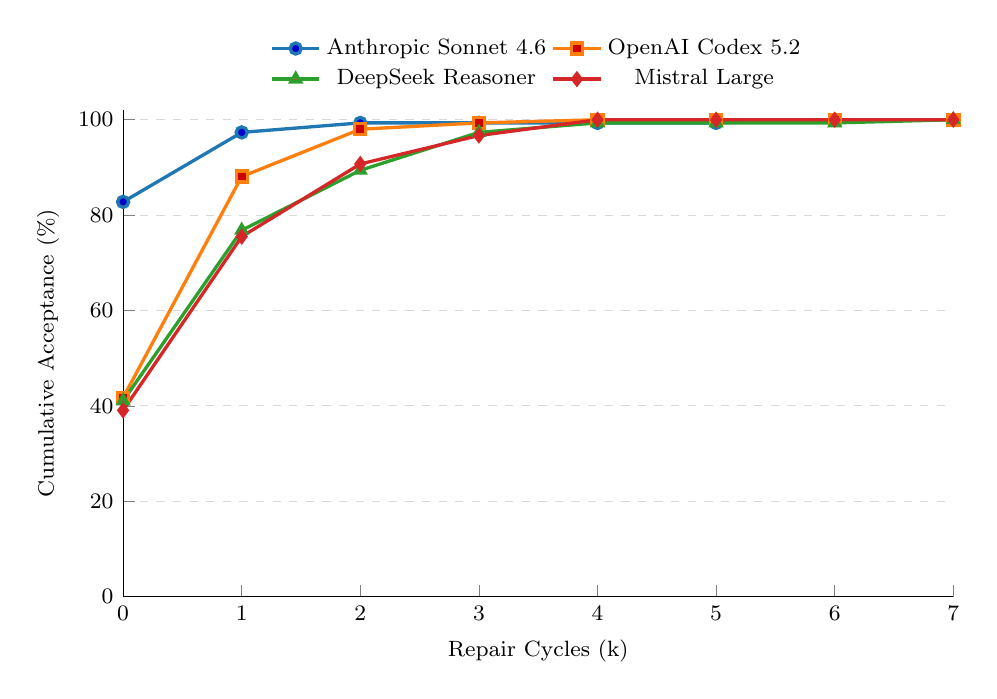
\begin{tikzpicture}
\begin{axis}[
    width=\columnwidth,
    height=0.64\columnwidth,
    xmin=0,
    xmax=7,
    ymin=0,
    ymax=102,
    xlabel={Repair Cycles (k)},
    ylabel={Cumulative Acceptance (\%)},
    xtick={0,1,2,3,4,5,6,7},
    ymajorgrids=true,
    xmajorgrids=false,
    grid style={dashed,gray!30},
    axis lines*=left,
    tick label style={font=\footnotesize},
    label style={font=\footnotesize},
    legend style={
        draw=none,
        font=\footnotesize,
        at={(0.5,1.02)},
        anchor=south,
        legend columns=2
    },
]
\addplot+[sonnetColor, very thick, mark=*] coordinates {
    (0,82.78) (1,97.35) (2,99.34) (3,99.34) (4,99.34) (5,99.34) (6,100.00) (7,100.00)
};
\addplot+[openaiColor, very thick, mark=square*] coordinates {
    (0,41.72) (1,88.08) (2,98.01) (3,99.34) (4,100.00) (5,100.00) (6,100.00) (7,100.00)
};
\addplot+[deepseekColor, very thick, mark=triangle*] coordinates {
    (0,41.06) (1,76.82) (2,89.40) (3,97.35) (4,99.34) (5,99.34) (6,99.34) (7,100.00)
};
\addplot+[mistralColor, very thick, mark=diamond*] coordinates {
    (0,39.07) (1,75.50) (2,90.73) (3,96.69) (4,100.00) (5,100.00) (6,100.00) (7,100.00)
};
\legend{Anthropic Sonnet 4.6,OpenAI Codex 5.2,DeepSeek Reasoner,Mistral Large}
\end{axis}
\end{tikzpicture}

\caption{Per-model cumulative production-validation acceptance versus repair cycles ($k$).}
\label{fig:cumulative_convergence_by_model}
\end{figure}

Figure~\ref{fig:cumulative_convergence_by_model} shows that single-shot starting points differ across models, but the trajectories compress rapidly once validator-guided repair begins. Despite different initial acceptance levels, all curves move quickly toward full acceptance within a small number of repair cycles. This pattern supports the model-agnostic control-signal interpretation: deterministic validator diagnostics drive the dominant convergence dynamics across backends.

\subsection{Statistical Reliability}
This subsection reports realized values for the convergence-reliability analysis defined in Section~3.6. Across the full campaign, $n=604$ prompt--model cases were evaluated, and eventual production-validation acceptance was observed in all cases ($x=604$, failures $=0$). Single-shot pass rate was 51.16\% (309/604), while pipeline pass rate was 100.00\% (604/604).

Under the Bernoulli convergence model, the exact 95\% Clopper--Pearson lower confidence bound for convergence probability $p$ in the all-success case is $p_L=(\alpha/2)^{1/n}$ with $\alpha=0.05$ and $n=604$, giving $p_L=(0.025)^{1/604}\approx 0.9939$ (99.39\%)~\cite{clopper1934confidenceLimits}. Therefore, with 95\% confidence, convergence probability is at least 99.39\% for SysMBench-style prompts under the evaluated controller, validator, and backend configuration.

For failure probability $q=1-p$, the complementary one-sided 95\% binomial upper bound is obtained from $(1-q)^n=0.05$. Substituting $n=604$ gives $q_U=1-0.05^{1/604}\approx 0.00495$ (0.495\%). The large-$n$ approximation gives $q_U\approx-\ln(0.05)/604\approx 0.00496\approx 3/604$.

These reliability bounds are intentionally scoped to SysMBench-style prompt distributions under the evaluated configuration and do not claim universal convergence over arbitrary natural-language inputs. Because the validator-gated loop is monotonic (accepted cases terminate immediately) and repairs are guided by deterministic diagnostics, the observed reliability is consistent with a structural property of validator-in-the-loop control on this benchmark distribution.

\subsection{Grammar Validity vs Production Validity and Error Burden}
Beyond aggregate reliability, practical MBSE usability requires production validation acceptance in a modeling environment, not only grammar parsability. To quantify this operational gap, we compared first-iteration ANTLR parsing outcomes against first-iteration production validation outcomes for all 604 prompt--model cases.

\begin{table}[H]
\centering
\caption{First-iteration contingency between grammar parsing (ANTLR) and production validation acceptance (SysIDE), $n=604$.}
\label{tab:antlr_vs_production_contingency}
\begin{tabular}{lrrr}
\toprule
 & \multicolumn{1}{c}{SysIDE pass} & \multicolumn{1}{c}{SysIDE fail} & \multicolumn{1}{c}{Total} \\
\midrule
ANTLR pass & 309 & 60  & 369 \\
ANTLR fail & 0   & 235 & 235 \\
\midrule
Total      & 309 & 295 & 604 \\
\bottomrule
\end{tabular}
\end{table}

The first-iteration grammar pass rate was 369/604 (61.09\%), while the first-iteration production pass rate was 309/604 (51.16\%). Grammar-only passes occurred in 60 cases. This corresponds to 60/369 = 16.26\% of grammar-valid outputs and 60/604 = 9.93\% of all outputs. Grammar-level parsing overestimates production usability by 16.26\% among parseable artifacts. No cases were observed with production pass and grammar fail (0/604). Thus, grammar validity is strictly necessary but not sufficient for production-validation acceptance under the evaluated configuration.

First-iteration validator diagnostics totaled 2,209 errors, giving a mean of 2,209/604 = 3.66 errors per generated model, indicating that first-iteration outputs frequently contain multiple structural defects rather than isolated formatting errors. Restricting to failing first-iteration cases (295), the mean burden was 2,209/295 = 7.49 errors per failing model. Error burden was concentrated in \texttt{parsing-error} (1,144; 51.79\%) and \texttt{reference-error} (824; 37.30\%), which together account for 89.09\% of first-iteration errors. These results indicate that validator-gated repair is addressing multi-error structural artifacts and that grammar-level parsing alone would have admitted non-usable models into downstream workflows.

\subsection{Open-Source Dataset Release}
This campaign releases an open-source dataset of 604 generated SysMLv2 outputs (151 prompts $\times$ 4 model backends), together with run-level records, iteration histories, and validator diagnostics in the project repository~\cite{sysmbenchCompilerLoopRepo2026}. This provides a reproducible, inspectable benchmark-scale corpus for follow-on syntactic-reliability studies.
